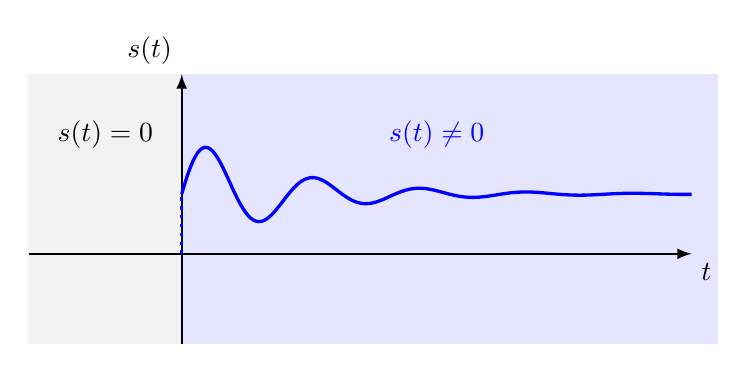
\begin{tikzpicture}
    \tikzstyle{signal}=[very thick,samples=201]
    \tikzstyle{recneg}=[white!95!black,fill=white!95!black]
    \tikzstyle{recpos}=[white!90!blue,fill=white!90!blue]
    \begin{axis}
    [   axis line style = thick,
	ticks=none,
        height=5cm,
        width=10cm,
        axis x line=center,
        axis y line=center,
        xmin=-3,
        xmax=10,
        ymin=-1.5,
        ymax=3.0,
        xlabel={$t$},
        ylabel={$s(t)$},
        xlabel style={below right},
        ylabel style={above left},
        clip=false,
    ]
    \draw[recneg] (axis cs:-3,-1.5) rectangle (axis cs:0,3);
    \draw[recpos]   (axis cs:0,-1.5) rectangle (axis cs:10.5,3);
    \draw[thick,-latex]   (axis cs:-3.0,0) -- (axis cs:10,0);
    \draw[thick,-latex]   (axis cs:0,-1.5) -- (axis cs:0,3);
    \addplot[black,domain=-3:0] {0};                                
    \addplot[signal,blue,domain=0:10] {sin(3*deg(x))*exp(-0.5*x)+1};
    \draw[dotted,very thick,blue] (axis cs:0,0) -- (axis cs:0,1); 
    \node[black] at (axis cs:-1.5,2.0) {$s(t)=0$};
    \node[blue] at (axis cs:5.0,2.0) {$s(t)\ne0$};
    \end{axis}
\end{tikzpicture}
